\section{Discussion of results}
\paragraph{Table}

\begin{center}
\resizebox{\textwidth}{!}{
\begin{tabular}{||c c c c c c||}
 \hline
 system of equations & method & demanded tolerance & error & iterations \\
 \hline
 task 3 system & Jacobi method & 10e-10 & 1.154375287358407e-10 & 38 \\
 \hline
 task 3 system & Jacobi method & 10e-10 & 5.770361548895147e-11 & 37 \\
 \hline
 task 3 system & Jacobi method & 3.202372833989376e-15 & 3.108624468950438e-15 & 53 \\
 \hline
 task 3 system & Gaussian-Seidel method & 10e-10 & 6.999102842719934e-10 & 19 \\
 \hline
 task 3 system & Gaussian-Seidel method & 1.776356839400250e-15 & 1.776356839400250e-15 & 30 \\
 \hline
 task 3 system & Matlab function & ? & 4.070144838902081e-15 & ? \\
 \hline
 task 2a) system & Jacobi method & 10e-10 & 6.955194519943778e-11 & 59 \\
 \hline
 task 2a) system & Jacobi method & 10e-10 & 1.699812218689508e-10 & 57 \\
 \hline
 task 2a) system & Jacob method & 3.202372833989376e-15 & 3.108624468950438e-15 & 84 \\
 \hline
 task 2a) system & Gaussian-Seidel method & 10e-10 & 5.311669113699570e-10 & 28 \\
 \hline
 task 2a) system & Gaussian-Seidel method & 1.538370149106851e-15 & 1.538370149106851e-15 & 42 \\
 \hline
 task 2a) system & Matlab function & ? & 3.662053438817790e-15 & ? \\
 \hline

\end{tabular}}
\end{center}
\subsection{Comparison based on table}
Gaussian-Seidel method takes less iterations, can achieve smaller error and works under smaller demanded tolerance, that being said Jacobi method has one crucial advantage - it can be run in parallel. That means that even when Jacobi method takes twice or thrice amount of iteration us Gaussian-Seidel one if we just run it in paraller we can diminish this difference. In the examples we worked in, just two jacobi method running in paraller provide us with similar amount of iterations per one process as in Gaussian-Seidel one, and three or more processes give the edge to Jacobi method. With modern CPU's with at least 5 cores and correct implementation of algorithm, jacobi method reigns supreme.

\newpage
\subsection{Convergence}
The biggest problem is of course the fact that those iterative methods do not work on every system of equation. Like the one from task 2b).
For Jacobi's method the matrix is convergent if it has strong diagonal dominance. \textbf{A}, i.e:
\begin{enumerate}
  \item \[ \| a_{ii} \| > \sum^n_{j=1, j \neq i} \|a_{ij} \| \]
  \item \[ \| a_{jj} \| > \sum^n_{i=1, i \neq j} \|a_{ij} \| \]
\end{enumerate}
For Gaussian-Seidel method the matrix is convergent if it has strong diagonal dominance \textbf{or} if the matrix \textbf{A} is symmetric and positivie definite.
\subsubsection{2b) task convergence }
Let's check strong diagonal dominance from matrix \textbf{A} from task 2b) in matlab:
\begin{simplechar}

\hyperlink{function_3_dominant}{Code for checking if matrix is diagonally dominant}
\\

checkIfDiagonallyDominant(matrixB(10)) returns '0', therefore matrix from task 2b) will \textbf{not} converge. And as expected it does not work when put in my jacobiLoop function.
\subsubsection{Iterations as function of size of Matrix}
\hyperlink{function_3_plot}{Code for creating plot}
I have used matrix from task 2a), demanded tolerance equal to 10e-10, and max size of matrix equal to 500. for both methods
\begin{center}
   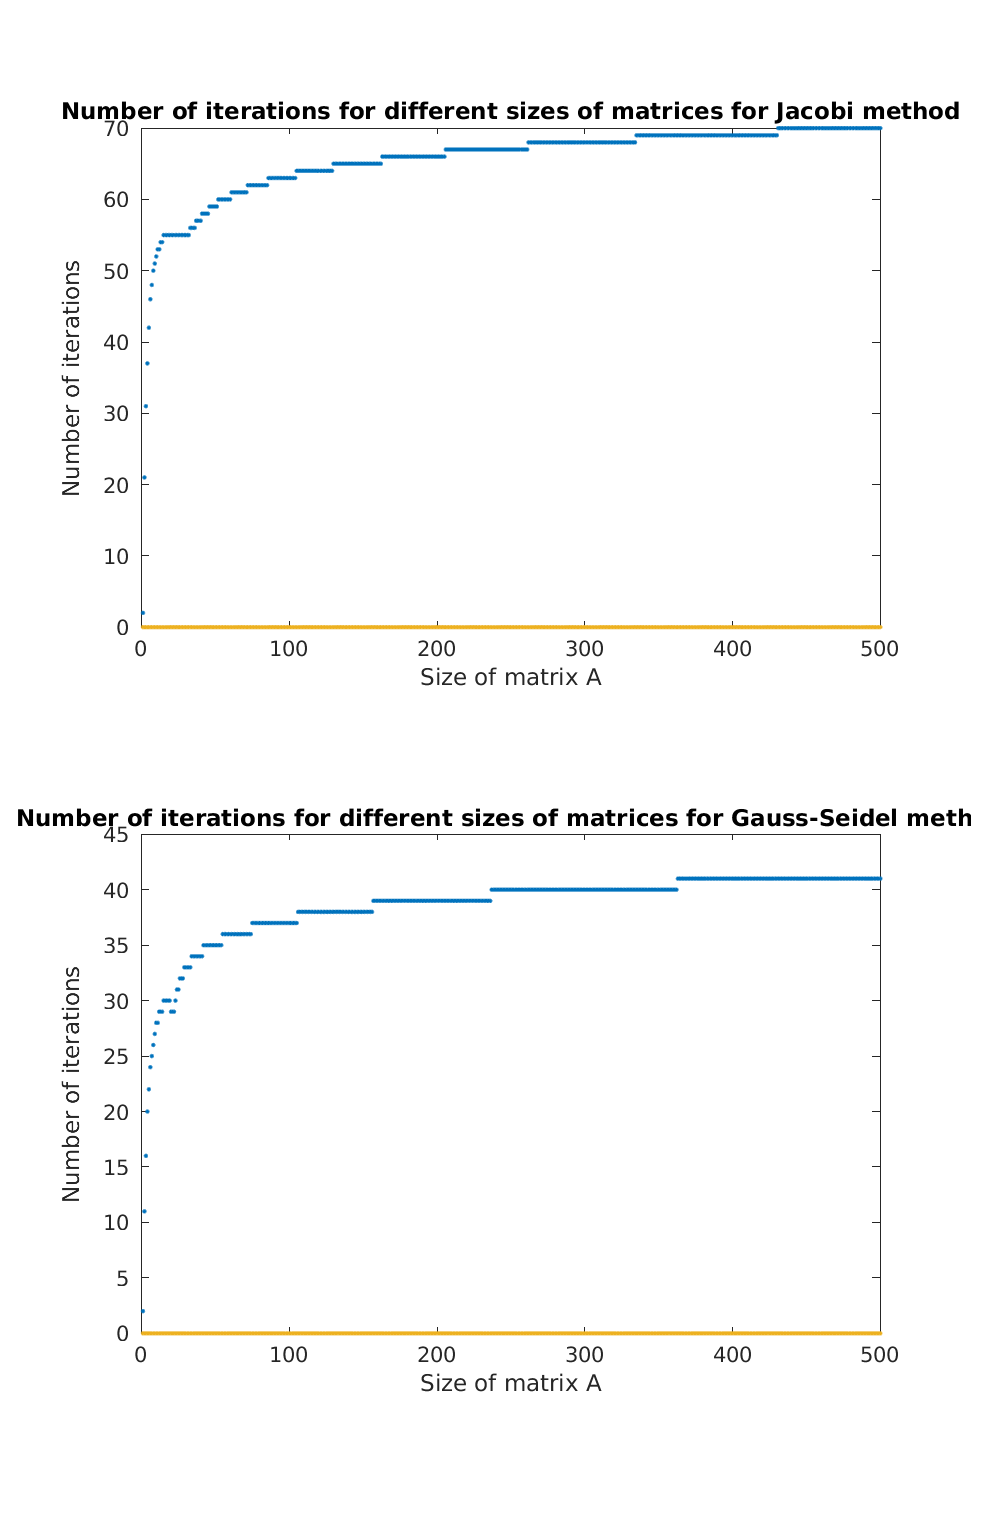
\includegraphics[scale=0.75]{iterations.eps}
\end{center}
Gauss Seidel method again requires fewer iterations, around half the amount for Jacobi method. For both methods function of number of iterations acts like logarithmic function. Therefore we can assume that for big matrices required number of iterations will \textbf{not} change rapidly.

\chapter{Problem 4 - QR method of finding eigenvalues}

